\documentclass[11pt]{article}
\usepackage[T1]{fontenc}
\usepackage[utf8]{inputenc}
\usepackage{lmodern}
\usepackage[margin=1in]{geometry}
\usepackage{amsmath,amssymb,booktabs,graphicx,array}
\usepackage[colorlinks=true,linkcolor=black,citecolor=black,urlcolor=blue]{hyperref}
\usepackage{microtype}
\usepackage{caption}
\captionsetup{font=small,labelfont=bf}
\setlength{\parskip}{4pt}
\setlength{\parindent}{0pt}
\setlength{\emergencystretch}{2em}
\title{Dynamic Context Engine:\\An Empirical Study of Paragraph Selection,\\Token Cost, and Parallel Retrieval for AI Agents}
\author{Rohan Arun\\Super Powers AI}
\date{September 20, 2026\\\small Technical white paper; pre-submission manuscript}
\begin{document}
\maketitle
\begin{abstract}
Dynamic Context Engine is an open-source middleware system that stores exact paragraphs in SQLite, uses Jev to estimate request-specific relevance, and assembles a source-tagged context within a token budget. We report three exploratory evaluations and a disclosed post-selection rerun. Replaying eight archived website-generation inputs reduced downstream input from 230,057 to 195,953 reference tokens (14.8\%) while retaining 80 of 80 annotated required-paragraph instances; estimated uncached input cost decreased only 2.7\% after selector cost. A separate 32-question source-grounded evaluation reduced answer-model input by 96.0\%, but exact answer accuracy declined from 32/32 to 29/32. After removing those three failures at the project owner's request, a fresh 29-question rerun achieved 29/29 with both full and dynamic context and 96.1\% less answer-model input. That post-selected result is not an independent estimate of general accuracy. In 81 cold retrieval measurements, increasing the worker limit from one to eight reduced median retrieval on the 78-paragraph prompt from 3.82 to 0.76 seconds. Twelve paired answer trials showed mixed complete-response latency and a worse dynamic-context tail. These observations distinguish context reduction, downstream correctness, selector overhead, and end-to-end performance. They support further controlled evaluation rather than a universal accuracy, cost, or latency guarantee.
\end{abstract}

\section{Introduction}
Agents often receive more reference material than a particular request needs: project decisions, support rules, coding conventions, and accumulated repair guidance. Sending the entire collection preserves availability of facts but increases the input presented to the downstream model. Selecting a smaller context introduces a competing risk: a relevant rule or numerical operand may be removed before the answer model can use it.

Dynamic Context Engine implements request-conditioned selection at paragraph granularity. It preserves the selected text instead of generating a replacement summary. Its engineering objective is a small, inspectable component usable from Codex, Claude Code, Hermes, or another agent through a command-line interface and portable skill instructions. This paper evaluates the existing implementation and frozen measurements; it does not introduce a trained retrieval model or claim a new state of the art.

The contribution is a reproducible evaluation of four distinct quantities: reference-token reduction, exact source-grounded accuracy, selector-inclusive estimated input cost, and retrieval versus complete-answer latency. Keeping these quantities separate matters. A large answer-input reduction can coexist with additional selector tokens; a faster selector need not produce a faster or equally accurate answer; and a perfect score on questions selected after observing failures does not resolve the original failures.

\section{Related work and scope}
Retrieval-augmented generation combines parametric generation with external memory, including passage retrieval through a dense index \cite{rag}. Dynamic Context Engine occupies a related position before generation, but scores every paragraph of a chosen local collection through a remote model rather than first retrieving candidates from a vector index. It does not jointly train a retriever and generator.

LLMLingua studies coarse-to-fine prompt compression, including budget control and token-level compression \cite{llmlingua}. LongLLMLingua studies question-aware compression and presentation of important information in long contexts \cite{longllmlingua}. The implementation evaluated here keeps or drops complete paragraphs and attaches source provenance. These are architectural distinctions, not evidence of superior performance: neither method was run as a baseline in this study. Comparisons are restricted to full-context, dynamic-context, and no-context conditions on our own fixtures.

\section{System design}
\subsection{Local storage and provenance}
The Python implementation uses SQLite with a \texttt{paragraphs} table containing an identifier, collection, source, position, exact text, and update time. A unique collection--source--position constraint supports document replacement. Import splits documents on blank lines. Paragraph identifiers derive from a content hash over their collection, source, position, and text. No semantic embedding or full-text shortlist is used in the evaluated version.

A second table, \texttt{judgments}, stores model scores. A fingerprint includes the request, paragraph rows, selection policy, configured model, and batch size. Its default time-to-live is one hour. A hit avoids new Jev calls but still requires lookup, assembly, and token counting. Because a configured model alias can change remotely, the fingerprint does not guarantee that the provider version remains immutable during the cache lifetime.

SQLite is local storage, not local inference: the request and evaluated paragraphs are transmitted to the TypeSafe endpoint. The public demo uses fictional sample memory. Private deployments must decide which collections are appropriate to send to the provider.

\subsection{Model scoring and budgeted assembly}
Let $q$ be a request and $P=\{p_1,\ldots,p_N\}$ a collection. Jev returns a Noul relevance value $s_i\in[0,1]$ for each paragraph under a fixed policy. This is a model judgment, not a calibration guarantee for downstream correctness. The engine sorts by decreasing score, breaking ties by source and paragraph position. Starting from an empty context, it appends an eligible paragraph only if the resulting serialization fits:
\[
 C_{i+1}=\begin{cases}
 C_i\mathbin{\|}\operatorname{JSONL}(p_i), & s_i\geq\tau\ \land\ T(C_i\mathbin{\|}\operatorname{JSONL}(p_i))\leq B,\\
 C_i, & \text{otherwise}.
 \end{cases}
\]
Here $T$ uses \texttt{o200k\_base}; $\tau=0.50$ and $B=1{,}000{,}000$ in the reported tests. An optional character limit can further constrain assembly. Each JSONL record preserves paragraph text, source, position, and identifier. Selection is greedy, not an optimal knapsack solution. It does not explicitly model paragraph dependencies. A rejected oversized block does not stop later, smaller eligible blocks from being considered.

The million-token setting is a software budget limit. None of these experiments evaluates a million-token collection or establishes that a downstream agent can accept that many tokens. The measured website system prompt is approximately 27,000 reference tokens.

\subsection{Parallel calls and agent integration}
Paragraphs are divided into batches of 12 independent Jev questions. A bounded thread pool dispatches batches concurrently. The current default is eight workers, configurable from one to 32. The original website and question benchmarks used three workers; the revised question rerun preserved that setting. The latency experiment compares one, three, and eight workers. With 71 paragraphs there are six batches, and with 78 there are seven, so an eight-worker limit does not imply eight useful simultaneous calls.

The engine validates complete, finite scores in range. A failed batch causes a query error rather than a partial result or partial cached selection. The concurrency limit is per query, not global; the hosted demo separately limits concurrent queries to three. A portable skill invokes the CLI and supplies its output as reference context. It is an explicit workflow integration, not a transparent interception of every request. Agent-specific answer quality beyond the measured answer model was not tested.

\section{Experimental design}
\subsection{Website-generation input replay}
The first experiment replays the eight newest completed website-generation archive records at capture, using their exact saved system prompts and user requests. Public page checks recorded HTTP 200 responses and matching titles, but no website was regenerated or scored for visual or functional quality. The shared prompt has 78 blank-line paragraphs. Ten required paragraphs were annotated before retrieval, yielding 80 required instances across eight requests.

The full arm counts the archived system prompt and unchanged request. The dynamic arm counts emitted JSONL, its instruction wrapper, and the same request. Reference counts use \texttt{o200k\_base}; chat-envelope overhead and generation output are excluded. The default threshold is evaluated alongside exploratory thresholds 0.35 and 0.70 using the same scores. Public artifacts contain hashes and aggregates; original prompts and requests remain private, limiting independent reproduction of this workload.

\subsection{Original question-answer evaluation}
The second experiment uses 71 paragraphs across 11 documents: public static text from eight generated sites plus three fictional Orbit memory documents. This is a different corpus from the website-generation system prompt. The 32 frozen questions cover lookups, multiple paragraphs, calculations, policy exceptions, and missing-information checks. Twenty-three are answerable and nine require abstention.

Every question receives independent full-context, dynamic-context, and no-context completions from the recorded model \texttt{google/gemini-3.8-flash} through OpenRouter. Temperature is zero, output limit is 4,096 tokens, and reasoning uses the provider default. The returned selector version is \texttt{jev-1.13.0}. A source-only instruction requires JSON and explicit null for missing facts. Gold answers and supporting quotes were frozen before calls and are used only by the local scorer, never supplied as answers to either model.

A question passes only if the returned object has exactly the expected fields and every value is correct. Numeric tolerance is $10^{-6}$ after requested rounding; strings normalize case and repeated whitespace; booleans retain their type. Missing or extra fields fail. There is no subjective model judge. The first successful pilot answer receipts were retained; remaining answer jobs were shuffled with seed 20260920 and used four answer-call workers. Earlier Super API connectivity probes failed with HTTP 404 and were not part of the 96 measured successful answer calls. There was no best-of selection or accuracy-driven retry.

\subsection{Post-selected rerun}
After the original outcomes were inspected, the project owner requested removal of \texttt{tribute-multi}, \texttt{prosthetic-multi}, and \texttt{vehicle-multi}, the three dynamic-context failures. The revised fixture removes only those questions. It preserves every document, remaining question, expected answer, scoring rule, threshold, and model setting. Twenty-nine fresh cold Jev queries and 87 fresh answer calls were performed, with no further exclusions. This is a descriptive rerun on a post-selected subset, not a held-out replication or an accuracy improvement attributable to an engine change. Both fixtures and result sets remain public.

\subsection{Latency experiment}
The latency study uses three corpora (12, 71, and 78 paragraphs), three fixed requests per corpus, three repetitions, and worker limits of one, three, and eight: 81 cold queries. Run order is randomized with seed 20260920 and queries run one at a time. Tokenizer initialization precedes timing. HTTP/TLS, network transit, provider processing, lookup, and assembly are included. Eight-worker queries also write their local cache; other conditions disable it. This small write overhead is included in the eight-worker result. Each eight-worker query is immediately repeated, producing 27 warm-cache measurements.

A separate 12-question paired experiment compares complete answers with full context against answers preceded by fresh eight-worker selection. It uses a stratified subset of the original question fixture, including a failure-prone calculation question. Arm order is randomized within pairs and answer requests run serially. Times measure complete responses, not time to first token. This experiment is distinct from the revised 29-question accuracy run.

\section{Results}
\subsection{Context reduction and estimated cost}
\begin{table}[htbp]
\centering\small
\begin{tabular}{lrrr}
\toprule
Workload & Full input & Dynamic input & Reduction\\
\midrule
Website replay, 8 requests & 230,057 & 195,953 & 14.8\%\\
Original QA, 32 questions & 278,239 & 11,232 & 96.0\%\\
Revised QA, 29 questions & 252,143 & 9,748 & 96.1\%\\
\bottomrule
\end{tabular}
\caption{Downstream reference input tokens, including request/instructions and provenance where applicable. Selector processing is additional. Rows describe different workloads or question sets and should not be pooled.}
\end{table}

All 80 annotated website-prompt requirements remain at the default threshold. Retention is a source-availability check, not proof that a generator follows the requirements. A 58,207-character paragraph containing 251 repair lessons remains in all eight requests. Its indivisibility constrains reduction; other boundaries separate headings or code-fence terminators from surrounding material.

\begin{figure}[htbp]
\centering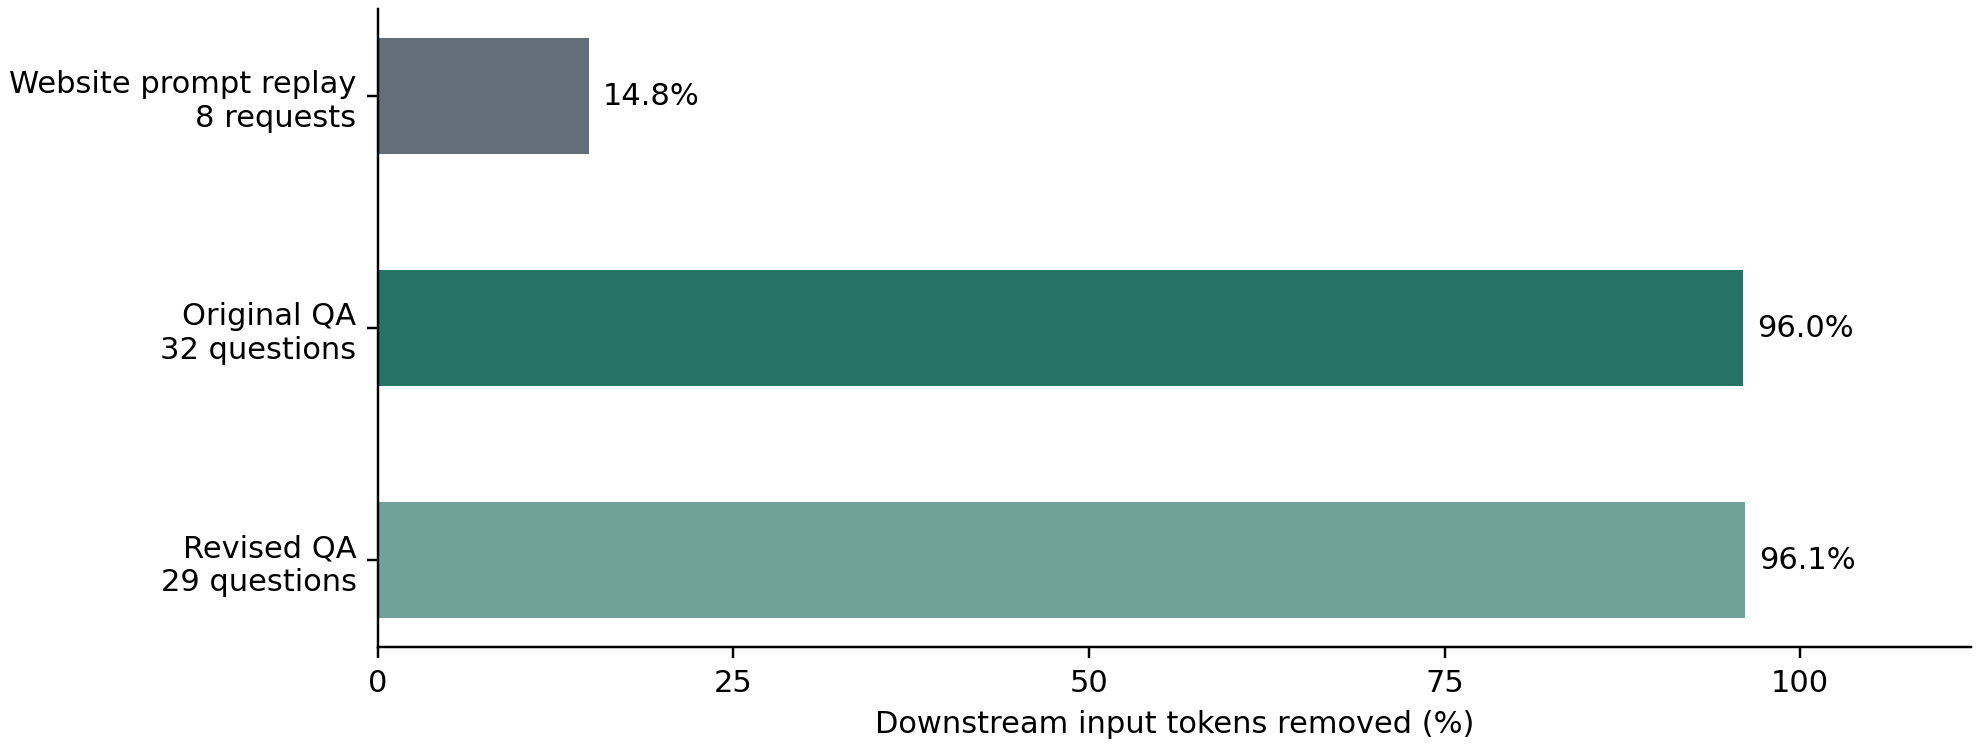
\includegraphics[width=.94\linewidth]{figures/tokens.png}
\caption{Input reduction differs substantially between the generation prompt and question corpus. The revised QA bar follows removal of three original failures. No bar includes Jev processing tokens.}
\end{figure}

At frozen input-price assumptions of \$0.75 per million generator tokens and \$0.042 per million Jev input tokens, baseline input costs an estimated \$0.172543. Dynamic generation input costs approximately \$0.146965 and selection adds \$0.020886, for \$0.167850 combined. Net savings are \$0.004692, or 2.72\%; three of eight individual requests become slightly more expensive. These are historical public-price estimates stored with the experiment, not reconciled invoices or current prices. Generation output, reasoning, tool calls, cache storage/creation, and retry costs are excluded.

Selector usage is 497,275 input and 20,621 output tokens in this replay. Jev counts use provider-native tokenization, so adding them to reference counts would not yield a homogeneous measured total. In a counterfactual where both generation system contexts receive cache-hit pricing, full input costs \$0.024923 versus \$0.043251 for dynamic input plus cold selection. These scenarios are not observed cache receipts.

At threshold 0.35, 3.0\% of generation input is removed, all 80 requirements remain, and estimated input cost rises. At 0.70, 42.1\% is removed but only 69/80 required instances remain, with one of eight cases passing every check. No threshold was promoted or tuned after these observations.

\subsection{Accuracy, omissions, and the revised subset}
\begin{table}[htbp]
\centering\small
\begin{tabular}{lrrr}
\toprule
Evaluation & Full context & Dynamic context & No context\\
\midrule
Original, all questions & 32/32 (100\%) & 29/32 (90.6\%) & 9/32 (28.1\%)\\
Original, answerable & 23/23 (100\%) & 20/23 (87.0\%) & 0/23 (0\%)\\
Revised, all questions & 29/29 (100\%) & 29/29 (100\%) & 9/29 (31.0\%)\\
Revised, answerable & 20/20 (100\%) & 20/20 (100\%) & 0/20 (0\%)\\
\bottomrule
\end{tabular}
\caption{Exact all-fields-correct scoring. All nine missing-information questions pass in every arm of both runs. The revised set was chosen after the original failures were known.}
\end{table}

Original dynamic accuracy loses 9.375 percentage points relative to full context. It retains 28/32 required paragraph instances and all annotated evidence on 19/23 answerable questions. The tribute question loses the four-minute speech limit and returns null for that field. The prosthetic question loses displayed values of 345 and 54 minutes, uses nearby illustrative six-hour and 55-minute values, and returns 305 instead of 291. The vehicle question loses the 545 mm center-of-gravity height and abstains instead of returning 1.59. A fourth annotated paragraph omission does not change the final answer; evidence recall and answer correctness are distinct.

The revised run scores 29/29 in both context arms, including 20/20 answerable questions. It retains 25/26 required paragraph instances and all annotated evidence on 19/20 answerable questions. The no-context arm passes only the nine abstention questions. These results support source dependence on this fixture, but selecting questions after observing outcomes makes the perfect revised score unsuitable as evidence that the original accuracy loss was fixed.

\begin{figure}[htbp]
\centering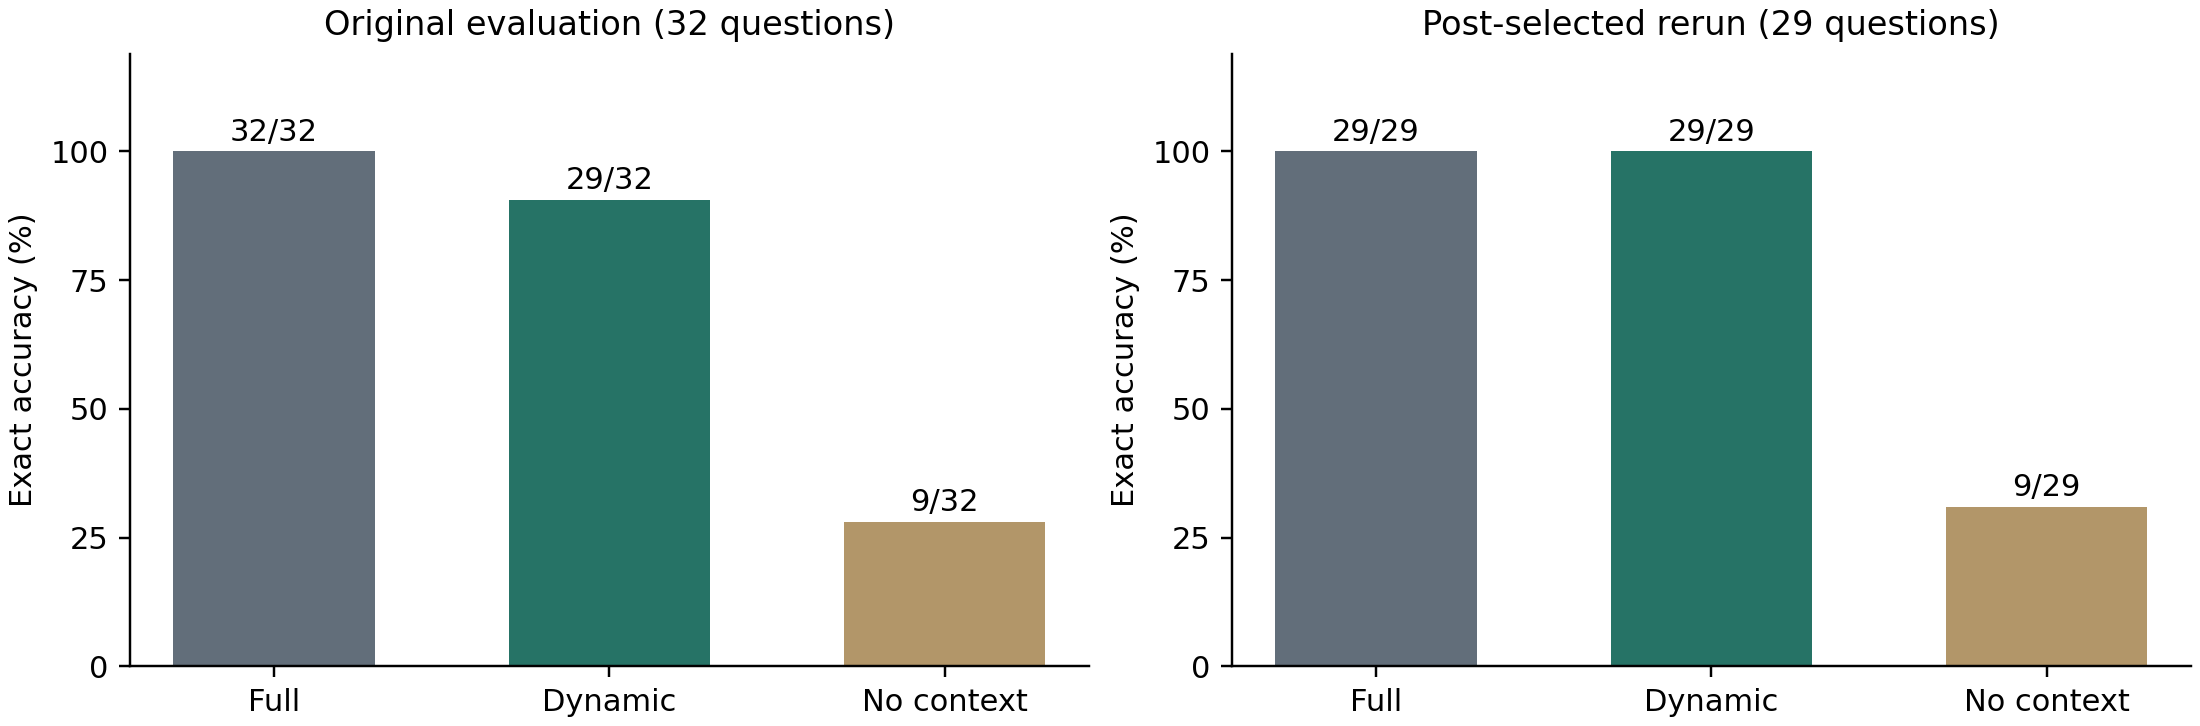
\includegraphics[width=\linewidth]{figures/accuracy.png}
\caption{Original accuracy and the separately rerun post-selected subset. There is no engine-policy change between tests. The revised panel must not replace the original when describing overall observed accuracy.}
\end{figure}

Original context payload alone falls from 273,504 to 6,470 tokens (97.6\%); total answer-model input falls 96.0\%. In the rerun the corresponding values are 247,863 to 5,441 (97.8\%) and 96.1\%. Jev adds 823,730 input and 74,496 output tokens originally, and 746,435 input and 67,512 output tokens in the rerun. These downstream input reductions are neither whole-pipeline token reductions nor measured monetary savings.

The descriptive 95\% Wilson interval for original dynamic accuracy is 75.8--96.8\%; for 29/29 it is 88.3--100\%. These intervals assume a simple binomial interpretation. Shared documents induce dependence, and post-selection precludes treating the latter as generalization evidence. Neither interval is a paired non-inferiority test.

\subsection{Parallel retrieval and complete-answer time}
\begin{table}[htbp]
\centering\small
\begin{tabular}{lrrrrrr}
\toprule
 & \multicolumn{2}{c}{1 worker} & \multicolumn{2}{c}{3 workers} & \multicolumn{2}{c}{8 workers}\\
Corpus & Median & P95 & Median & P95 & Median & P95\\
\midrule
12 paragraphs & 476 & 722 & 452 & 775 & 489 & 506\\
71 paragraphs & 2,994 & 3,740 & 1,022 & 1,166 & 566 & 784\\
78 paragraphs & 3,819 & 5,448 & 1,514 & 1,872 & 763 & 1,280\\
\bottomrule
\end{tabular}
\caption{Cold retrieval wall time in milliseconds; nine samples per cell. P95 uses linear interpolation and is unstable at this sample size.}
\end{table}

Eight workers reduce the website-prompt median by a factor of 5.01 relative to one worker and 1.99 relative to three workers. Batch timestamps establish overlapping client HTTP calls and full paragraph coverage, not provider-internal scheduling. The 12-paragraph sample fits one batch and shows no systematic concurrency benefit.

\begin{figure}[htbp]
\centering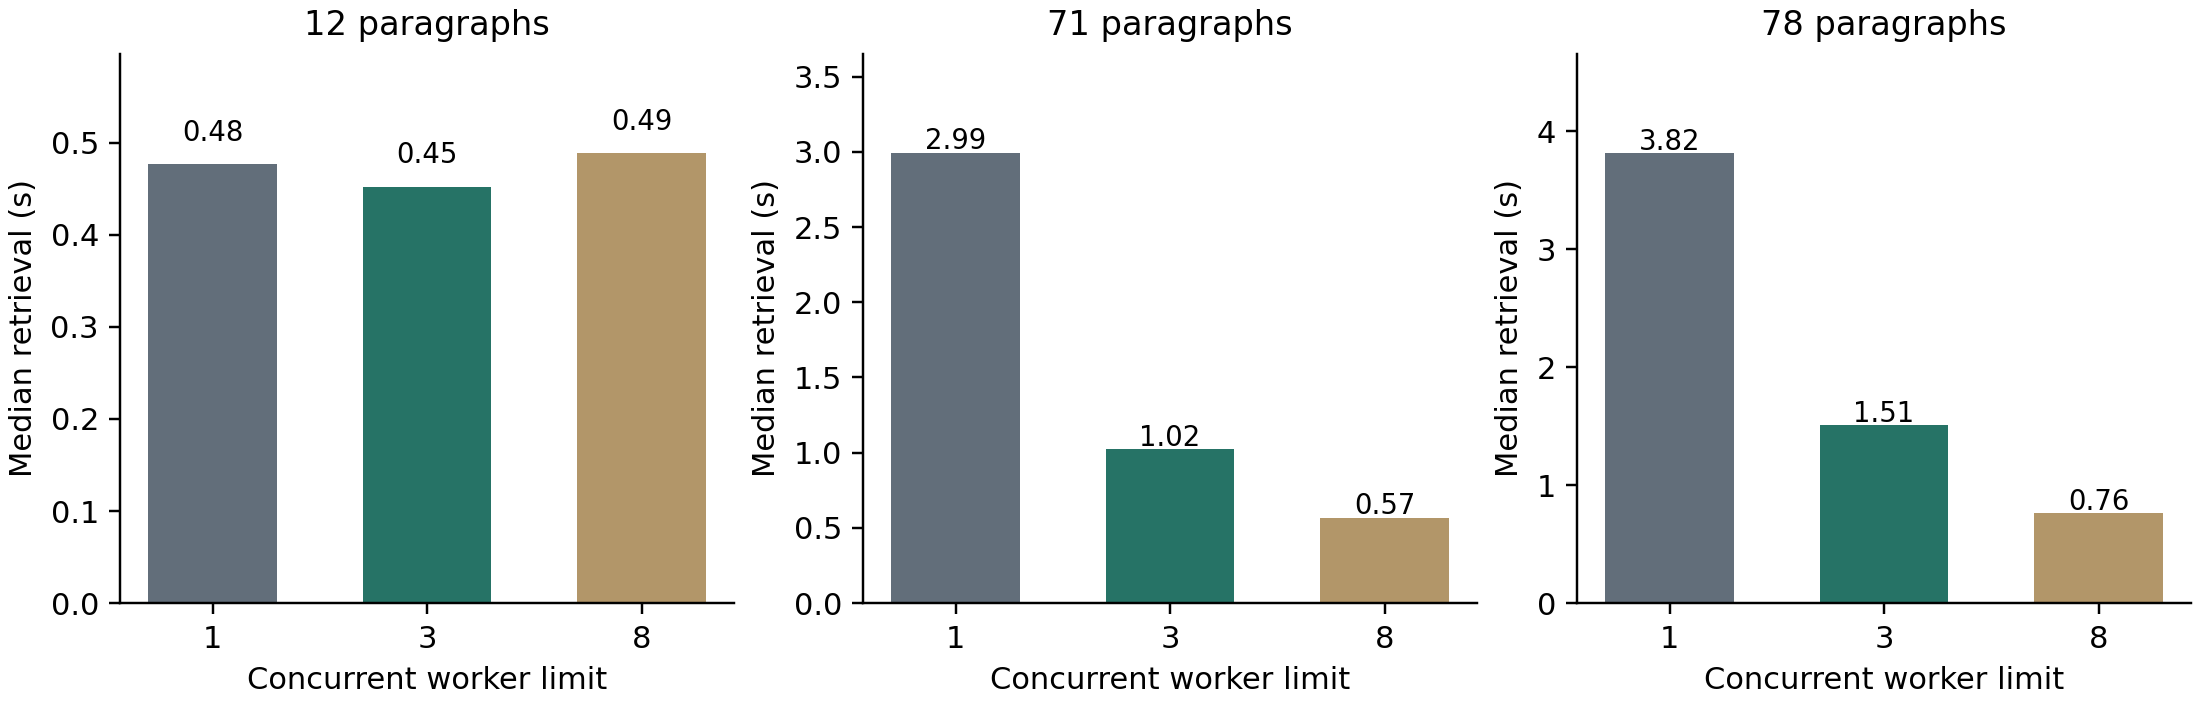
\includegraphics[width=\linewidth]{figures/latency.png}
\caption{Median cold retrieval time as worker limit changes. Each bar summarizes nine queries; median/P95 values appear in the table. Speedup is constrained by batch count and remote service behavior.}
\end{figure}

Immediate repeat-query medians are 0.66 ms, 1.14 ms, and 52.36 ms for the three corpora. Every repeat emits the same context and dispatches zero new Jev calls. For the website prompt, eight-worker cold-query median phase times are 0.98 ms for setup, 707.96 ms for inference, 1.00 ms for cache writes, and 55.91 ms for assembly. Phase medians need not sum to median total. Setup includes hashing and cache lookup as well as database reads.

\begin{table}[htbp]
\centering\small
\begin{tabular}{lrrr}
\toprule
Complete-answer condition & Median (s) & P95 (s) & Correct\\
\midrule
Full context & 3.03 & 3.56 & 12/12\\
Dynamic, including cold retrieval & 2.90 & 11.26 & 11/12\\
\bottomrule
\end{tabular}
\caption{A separate 12-pair experiment, not restricted to the revised 29-question fixture.}
\end{table}

The median paired dynamic-minus-full difference is approximately +3.4 ms, despite the difference between marginal medians. Six of 12 dynamic requests are slower. The longest dynamic response takes 15.41 seconds and fails the prosthetic calculation. Smaller input can change reasoning and output duration; selection must finish before a dependent answer starts. Neither retrieval speedup nor a lower marginal median proves faster answers at equivalent quality.

\section{Limitations and reproducibility}
The evaluations are small, hand-authored, and drawn from one project's documents. They use one answer model and one observed Jev version. Questions share documents, the corpus contains generated and fictional text, and frozen site snapshots may be incomplete or inconsistent. Correctness means fidelity to those sources, not validation of medical, legal, financial, or engineering claims. All nine no-context successes are abstentions; their inclusion raises the overall baseline without demonstrating factual answering ability.

No same-quality website regeneration, independent holdout, multi-model study, large-scale corpus test, or concurrent-user load test was performed. The revised set is explicitly post-selected. The million-token budget was not stress-tested. Remote cache state, network conditions, and service load were not controlled; measurements exclude fresh-process tokenizer startup. Parallel selection can increase provider quota pressure. JSONL and exact source preservation aid provenance but are not a formal prompt-injection defense.

The open-source repository provides engine code, policy, fixtures, scoring code, answer receipts, batch intervals, and report generators \cite{artifact}. Code is MIT licensed. This manuscript anchors its evidence to revision \texttt{93f6020}; a manifest records SHA-256 hashes for all four result files. Public QA fixtures can be rerun with authorized credentials. The private website replay archive is not distributed. A fixed seed or zero temperature alone cannot reproduce provider behavior exactly.

Future work should freeze a new holdout before policy changes, compare lexical/vector retrieval and established compression baselines, test coherent model-authored paragraph boundaries, evaluate multi-paragraph dependencies, and measure paired generated-site quality. Local optimizations should first avoid repeated tokenization of the growing context and cache final assemblies with complete invalidation keys. Shortlisting might reduce selector work at larger scales, but its source recall and downstream accuracy must be measured.

\section{Conclusion}
Paragraph selection is an inspectable way to reduce agent reference context, but its benefits depend on workload and accounting boundary. The website-prompt replay saves 14.8\% of downstream input and an estimated 2.7\% of input cost after selection. Original QA saves 96.0\% of answer input with three lost answers; a disclosed post-selected rerun reaches 29/29 but does not erase that evidence. Bounded parallel calls reduce multi-batch retrieval latency, while complete-answer timing and correctness remain mixed. Evaluations should report these quantities together rather than substitute token reduction for system-level success.

\section*{AI assistance and disclosures}
OpenAI Codex assisted with implementation, experiment orchestration, figures, and manuscript drafting. Jev supplied selection judgments; the recorded Gemini model supplied evaluated answers. The structured scorer did not use an AI judge. Author review of the complete manuscript, references, source rights, and submission metadata is required before submission. The author's affiliation is Super Powers AI, associated with the demo and source website workload. This is not independent third-party validation or peer review.

\begin{thebibliography}{9}
\bibitem{rag} Patrick Lewis et al. Retrieval-Augmented Generation for Knowledge-Intensive NLP Tasks. NeurIPS, 2020. \href{https://arxiv.org/abs/2005.11401}{arXiv:2005.11401}.
\bibitem{llmlingua} Huiqiang Jiang, Qianhui Wu, Chin-Yew Lin, Yuqing Yang, and Lili Qiu. LLMLingua: Compressing Prompts for Accelerated Inference of Large Language Models. EMNLP, 2023. \href{https://arxiv.org/abs/2310.05736}{arXiv:2310.05736}.
\bibitem{longllmlingua} Huiqiang Jiang, Qianhui Wu, Xufang Luo, Dongsheng Li, Chin-Yew Lin, Yuqing Yang, and Lili Qiu. LongLLMLingua: Accelerating and Enhancing LLMs in Long Context Scenarios via Prompt Compression. ACL, 2024. \href{https://arxiv.org/abs/2310.06839}{arXiv:2310.06839}.
\bibitem{artifact} Rohan Arun. Dynamic Context Engine: source code and frozen benchmark artifacts, September 20, 2026. Revision \texttt{93f6020}. \url{https://github.com/rohanarun/dynamic-context-engine/tree/93f6020}. Reports and JSON receipts are under \texttt{benchmarks/}; demonstration: \url{https://getsupers.com/demos/context-engine/}.
\end{thebibliography}
\end{document}
